\let\negmedspace\undefined
\let\negthickspace\undefined
\documentclass[journal,12pt,onecolumn]{IEEEtran}
\usepackage{cite}
\usepackage{amsmath,amssymb,amsfonts,amsthm}
\usepackage{algorithmic}
\usepackage{graphicx}
\graphicspath{{./figs/}}
\usepackage{textcomp}
\usepackage{xcolor}
\usepackage{txfonts}
\usepackage{listings}
\usepackage{enumitem}
\usepackage{mathtools}
\usepackage{gensymb}
\usepackage{comment}
\usepackage{caption}
\usepackage[breaklinks=true]{hyperref}
\usepackage{tkz-euclide} 
\usepackage{listings}
\usepackage{gvv}                                        
\usepackage[latin1]{inputenc}     
\usepackage{xparse}
\usepackage{color}                                            
\usepackage{array}                                            
\usepackage{longtable}                                       
\usepackage{calc}                                             
\usepackage{multirow}
\usepackage{multicol}
\usepackage{hhline}                                           
\usepackage{ifthen}                                           
\usepackage{lscape}
\usepackage{tabularx}
\usepackage{array}
\usepackage{float}


\begin{document}

\title{4.12.6}
\author{AI25BTECH11001 - ABHISEK MOHAPATRA}
{\let\newpage\relax\maketitle}
	 	\textbf{Question}:
The owner of a milk store finds that he can sell 980 litres of milk each week
at 14/litre and 1220 litres of milk each week at 16/litre. Assuming a linear
relationship between selling price and demand, how many litres could he sell weekly
at 17/ litre?

		\textbf{Solution:} 
Let the litres at 17/ litre be x.
Representing the data, Let
\begin{align}
\vec{A} = \myvec{980 \\ 14},
\vec{B} = \myvec{1220 \\ 16},
\vec{C} = \myvec{x \\ 17}
\end{align}

so as per the question these point lies on a line,
\begin{align}
	\Rightarrow rank\myvec{\vec{A}-\vec{B} & \vec{C}-\vec{B}}^\top = 1 
\end{align}

\begin{align}
	\Rightarrow \myvec{\vec{A}-\vec{B} & \vec{C}-\vec{B}}^T = \myvec{-240 & -2 \\ x-1220 & 1} 
\end{align}
\begin{align}
	\xleftrightarrow[]{C_1\xleftrightarrow[]{} C_2} \myvec{-2 & -240 \\ 1 & x - 1220}
\end{align}
\begin{align}
	\xleftrightarrow[]{R_2\rightarrow R_2 + \frac{1}{2}R_1} \myvec{-2 & -240 \\ 0 & x - 1340}
\end{align}

so for rank = 1, x = 1340.

1340 litres is the required answer.


Graph:
\begin{figure}[h!]
	\centering
	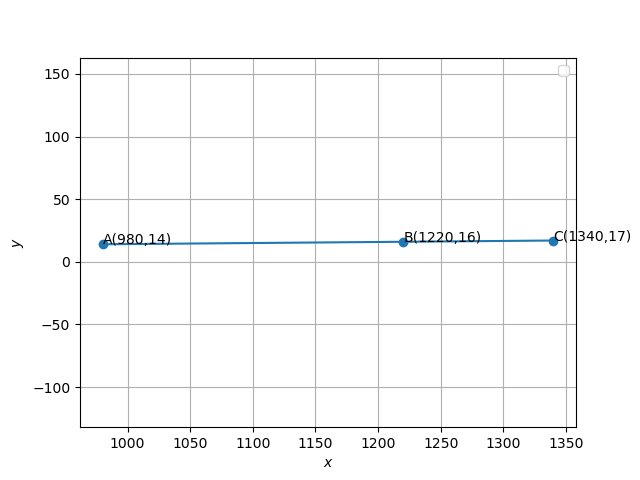
\includegraphics[width=0.7\linewidth]{fig1.png}
\end{figure}
\end{document}
